\documentclass[10pt,conference]{IEEEtran}
\usepackage[T1]{fontenc}
\usepackage{cite}
\usepackage{graphicx}
\usepackage{booktabs}
\usepackage{array}
\usepackage{listings}
\usepackage{xcolor}
\usepackage{tikz}
\usetikzlibrary{arrows.meta,positioning}
\usepackage[hidelinks]{hyperref}
\newcommand{\tool}{\textsc{Temporal Contracts}}

\lstdefinelanguage{JavaScript}{keywords={function,let,const,async,await,if,return},
  sensitive=true,morecomment=[l]{//},morestring=[b]"}
\lstset{basicstyle=\ttfamily\footnotesize,columns=fullflexible,keepspaces=true,
  breaklines=true,showstringspaces=false,frame=single,numbers=left,
  numberstyle=\tiny,numbersep=5pt,captionpos=b}
\title{Temporal Contracts: Reviewing Asynchronous and\newline Lifecycle Boundaries with Source Evidence}
\author{\IEEEauthorblockN{Author names to be supplied}
\IEEEauthorblockA{Affiliations and contact details to be supplied}}
\begin{document}
\maketitle
\begin{abstract}
An asynchronous operation can finish after its initiating view closes, and a synchronous notification can reenter an operation before it returns. Understanding these behaviors requires connecting execution boundaries to the state and effects whose validity they change. We present \tool{}, an interactive source review tool that organizes candidate temporal evidence into four questions: where execution crosses a boundary, what could change, which effects matter, and what requirements and protections apply. The analyzer extracts syntax events and bounded candidate relations from Python, JavaScript, TypeScript, and Vue scripts. A review workbench links these observations to archived source and records relation validity separately from protection sufficiency. Command-line, editor, and agent-facing interfaces share the same report archive. A reproducible synthetic demonstration contrasts an obsolete continuation with a reviewer-supplied epoch check under one controlled schedule. Both versions retain review hints, illustrating why hint disappearance is unsuitable as a repair criterion. The current evidence establishes this workflow and its implementation checks; independent measurements of comprehension benefit remain future work.

\end{abstract}
\begin{IEEEkeywords}
program comprehension, asynchronous programming, lifecycle, source evidence, developer tools
\end{IEEEkeywords}
\section{Introduction}
A panel starts a request, closes while the request is pending, and receives a result afterward. Whether the continuation should publish that result depends on the panel's requirements and on which operation still owns the output. The developer reviewing this code must answer a concrete question: which work becomes invalid at closure, and where must that invalidation constrain its continuation? Answering requires connecting the suspension point, lifecycle transition, publication, and protection.

Program comprehension during a change involves answering questions about relevant code and its relationships~\cite{sillito2006}. Temporal behavior adds a specific difficulty: a condition established before a boundary can cease to apply when execution resumes. Event-driven race detectors address related ordering problems using execution models~\cite{raychev2013}. A source review workflow can instead expose candidate relationships before the developer has reproduced an execution or established the application's validity requirements.

We organize this workflow around \emph{boundary review cards}. Each card links source references to four questions about a possible temporal relationship. A \emph{temporal contract} is an application requirement governing when an effect remains valid across execution or lifecycle boundaries. The analyzer selects candidate evidence; the reviewer establishes the requirement from repository documentation, implementations, or tests.

The tool provides three capabilities: (1) source extraction with explicit qualifications on candidate relations; (2) a four-question review interface that separates relation validity from protection sufficiency; and (3) shared, snapshot-based reports for command-line, editor, and agent-assisted review. The demonstration follows a pending request across panel closure and shows how the same review questions apply to an unguarded and a protected version.

\section{Tool Design and Implementation}
\label{sec:tool}
\subsection{From Source to Candidate Evidence}
The analyzer reads selected source files without executing the target project or calling a language model. Python's standard abstract syntax tree and Babel supply syntax events; the Vue single-file-component parser extracts inline script blocks before Babel analysis. Events retain original source positions, enclosing scopes, and selected syntax fields. Vue locations map back to the original component, and editor locations use UTF-16 columns.

Rules select candidate boundaries and effects from these events. Table~\ref{tab:rules} summarizes representative families. Some relations use lexical or import bindings; others use names or co-occurrence to nominate a review location. For example, a continuation and a cleanup method in one lexical namespace motivate a lifecycle question without establishing that they concern the same object. The report retains this qualification alongside the evidence.

\begin{table}[t]
\caption{Representative review clues and remaining semantic questions.}
\label{tab:rules}
\centering\footnotesize
\begin{tabular}{>{\raggedright\arraybackslash}p{0.18\columnwidth}>{\raggedright\arraybackslash}p{0.30\columnwidth}>{\raggedright\arraybackslash}p{0.34\columnwidth}}
\toprule
Family & Extracted clue & Reviewer checks \\
\midrule
Suspension & Effect-named call after \texttt{await} in one syntax block & Does the effect belong to valid work? \\
Lifecycle & Continuation and cleanup/close clues in a lexical unit & Do they share an instance and lifetime? \\
Notification & Member write before a direct callback candidate & Can the callback synchronously reenter? \\
Snapshot & Bounded local captured-value/output clues & Do capture and output have different lifetimes? \\
\bottomrule
\end{tabular}
\end{table}

\begin{figure}[t]
\centering
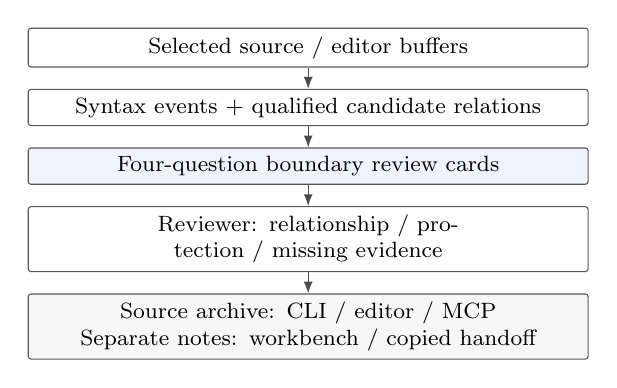
\begin{tikzpicture}[
 node distance=2.7mm,
 box/.style={draw=black!65,rounded corners=1pt,align=center,
   font=\footnotesize,text width=6.9cm,inner sep=3pt},
 flow/.style={-{Latex[length=1.5mm]},draw=black!70}]
\node[box] (src) {Selected source / editor buffers};
\node[box,below=of src] (syn) {Syntax events + qualified candidate relations};
\node[box,below=of syn,fill=blue!5] (card) {Four-question boundary review cards};
\node[box,below=of card] (human) {Reviewer: relationship / protection / missing evidence};
\node[box,below=of human,fill=black!3] (archive) {Source archive: CLI / editor / MCP\\Separate notes: workbench / copied handoff};
\draw[flow] (src)--(syn);
\draw[flow] (syn)--(card);
\draw[flow] (card)--(human);
\draw[flow] (human)--(archive);
\end{tikzpicture}

\caption{Conceptual review workflow and shared records in \tool{}. The source scan is archived before review; human notes are appended separately. Arrows connect review stages rather than program execution events.}
\label{fig:architecture}
\end{figure}

The scanner reports its analyzed files, skipped inputs, parser status, and scope limitations. Unsupported or unparsed material remains visible as incomplete coverage. Candidate direct-call links can extend a changed-file review to associated files; this expansion operates at file granularity.

\subsection{Four Questions and Two Judgments}
Each finding becomes a card with four fields. \emph{Boundary} references candidate waits, callbacks, notifications, or exits. \emph{Possible change} supplies a rule-specific question about state, identity, or ownership. \emph{Affected effects} references selected writes and effect calls, or requests further tracing when none was located. \emph{Requirement and protection} presents the review question and available guard or cancellation references. The projection classifies the finding's existing evidence; it does not recover an additional complete execution path.

Reviewers open the cited source and record two separate judgments. The first marks the candidate relationship as confirmed, dismissed, or uncertain. The second marks protection as sufficient, insufficient, or uncertain. A confirmed relationship can therefore be adequately protected. Reviewers can also record repository support and missing evidence. These annotations are appended to a report's notes, preserving the original scan.

\subsection{A Shared Report Archive}
The command-line interface, VS Code extension, and Model Context Protocol (MCP) server use one archive. A report ID identifies the captured source, analysis, parser metadata, and derived materials. The editor supports saved files and unsaved buffers; its scan archives the text actually analyzed. A later agent can read that report rather than assuming that a fresh disk scan captures the same input.

The workbench supports historical inspection, source navigation, annotations, and compatible before/after comparisons. Review-hint diagnostics are informational, and stale source locations are cleared after edits. Incomplete parsing produces a warning. MCP exposes scan, report lookup, paginated report/source reading, and comparison operations. Its report reads return frozen analysis materials; annotated review text is handed off using the workbench's copy action. MCP records prepared and transport-written responses, describing delivery rather than subsequent agent reasoning.

\section{Demonstration Scenario}
\label{sec:demo}
The demonstration uses a synthetic panel with an explicitly specified requirement: after \texttt{close}, work started in the previous epoch must not publish. The example isolates this requirement; it is not an independently collected repository incident. Listing~\ref{lst:panel} shows the protected version. Removing the capture of \texttt{started} and its comparison yields the unguarded version. The epoch protection is supplied by the reviewer.

\begin{lstlisting}[language=JavaScript,caption={Protected synthetic panel; the requirement is supplied with the example.},label={lst:panel}]
function createPanel(fetchValue, publish) {
  let epoch = 0;
  async function refresh() {
    const started = epoch;
    const value = await fetchValue();
    if (started !== epoch) return;
    publish(value);
  }
  function close() { epoch += 1; }
  return {refresh, close};
}
\end{lstlisting}

\paragraph{Locate and inspect.}
The presenter scans the unguarded version and opens its archived report. Three rules identify an effect after a wait, a continuation near a lifecycle boundary, and guard-state review. The first links the wait to the later \texttt{publish} call in source order. The lifecycle cards nominate the nearby close operation and state update. Their references support investigation; the presenter still checks that the returned operations share the panel's lexical state.

\begin{figure*}[t]
\centering
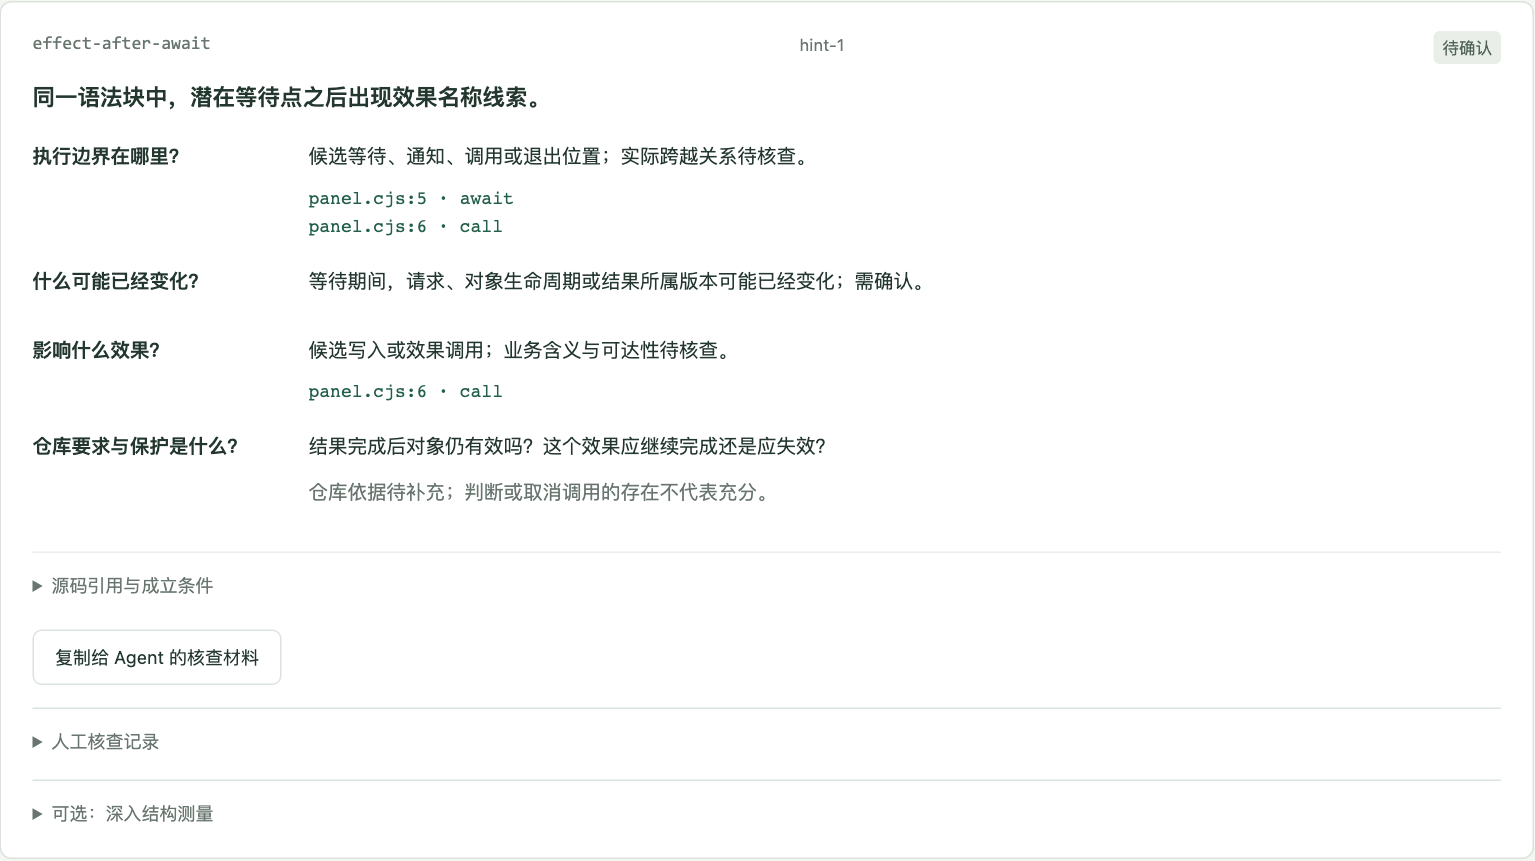
\includegraphics[width=0.90\textwidth]{figures/workbench.png}
\caption{Actual review card for the synthetic unguarded panel. The current interface uses Chinese labels; the four fields correspond to boundary, possible change, affected effects, and requirement/protection. Source references open the archived evidence.}
\label{fig:workbench}
\end{figure*}

\paragraph{Establish behavior.}
A separate replay script starts \texttt{refresh}, calls \texttt{close}, resolves the pending request, and awaits the continuation. The unguarded version publishes \texttt{old result}; the protected version produces no publication. This script executes the paper's synthetic programs independently of scanning. The observed behavior witnesses this particular schedule and stated requirement.

\paragraph{Review the protection.}
The presenter inspects the epoch comparison and records relation validity separately from protection sufficiency. The supplied capture script also saves an author-demonstration annotation for the unguarded report; this is a walkthrough record, not an independent judgment. Both versions retain the same three rule kinds. In the protected version, the guard-state card also references the conditional guard. The reviewer must determine why that guard connects the continuing work to its initiating epoch. A reduction in hint count would miss the relevant difference.

The session ends by comparing the archived versions. The comparison reports a changed guard-evidence finding while the rule kinds and total count stay constant. Reading either report through MCP retrieves that version's frozen materials; annotation history remains available in the workbench. The replay supplies the separate behavioral witness.

\section{Current Evidence and Limitations}
\label{sec:evidence}
\paragraph{Implementation checks.}
The current checkout passes 127 Python unit tests and nine extension runner tests on the development machine using Python 3.9.6. The suites cover extraction, scope separation, source positions, incomplete parses, archive consistency, and interface behavior. These counts describe regression checks, not independently confirmed defects. The two synthetic scans and their controlled replay are reproducible from the accompanying scripts. Editor-host and cross-platform installation validation remain outside this run.

\paragraph{Independent evaluation.}
The next evaluation will compare source navigation, raw findings, and four-question cards on held-out tasks. It will measure the correctness of boundary, identity, effect, and protection answers, followed by completion time and inspection effort. Task order and prior familiarity will be controlled. Dismissed and uncertain cards will remain in the analysis. Comprehension improvement remains an untested hypothesis.

\paragraph{Analysis scope.}
Name clues and lexical order leave API identity, aliasing, reachability, and complete callback dispatch unresolved. Vue support covers inline scripts; templates, reactive dependencies, and watcher scheduling remain outside the model. File-level change expansion can include unrelated functions and omit dynamic paths. A zero-hint result therefore cannot establish complete review coverage. Snapshot consistency supports source traceability, while semantic judgments still require repository evidence and, where appropriate, execution witnesses.

\section{Related Work}
Sillito et al. characterize questions developers ask during software evolution~\cite{sillito2006}. Our four questions specialize a question-oriented workflow to validity across temporal boundaries. Whyline derives questions about observed behavior from code and execution~\cite{ko2008}; \tool{} starts from source clues, with behavioral witnesses supplied separately.

Slicito supports interactive exploration by narrowing source scope and applying more precise analyses, including data-flow analysis and symbolic execution~\cite{slicito2025}. Our implementation organizes bounded temporal clues and reviewer judgments around a captured source version. EventRacer computes race coverage for event-driven programs~\cite{raychev2013}. Its execution-based ordering analysis addresses race detection; our cards expose questions about application-specific effect validity. The distinction concerns the review questions and the evidence available to answer them.

\section{Conclusion and Availability}
\tool{} organizes source evidence and separate reviewer judgments around effects that cross asynchronous and lifecycle boundaries. Its controlled demonstration illustrates a behavior change with persistent review hints. The current internal prototype requires a public source or binary release and installation instructions before submission. A demonstration video is planned. Independent evaluation will test the cards' comprehension benefit.

\section*{Acknowledgment}
OpenAI Codex assisted implementation inspection, manuscript drafting, demonstration scripts, and figure preparation. The authors remain responsible for verification.
\label{mainbodyend}
\clearpage
\bibliographystyle{IEEEtran}
\bibliography{references}
\end{document}
